\cotefile{161-6}
\scanpage{18}

\(u,v,w\)
\[
 \deleted{\unsure{u}}\,+v\cos i\tfrac{2\pi}{5}+w\sin i\tfrac{2\pi}{5}=p_i
 \qquad \boxed{0\leq i\leq4}
\]
\[
 \left\{\begin{aligned}
 &u\\
 &u\cos\alpha+p_i\sin\alpha\\
 &-u\cos\alpha-p_i\sin\alpha\\
 &-u
 \end{aligned}\right.
\]
\noindent
\figure{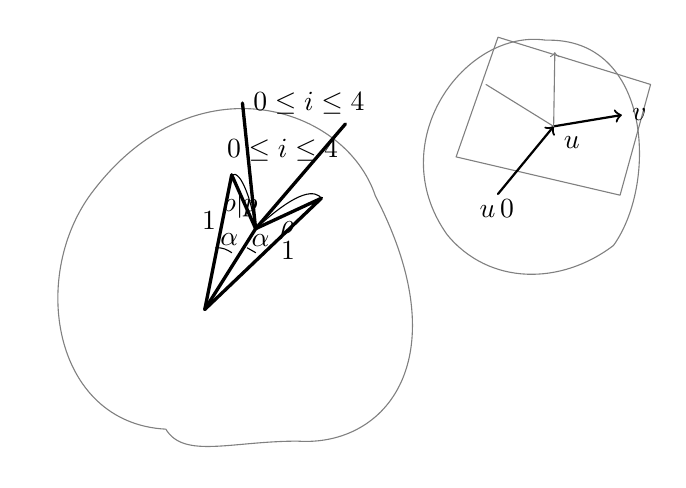
\begin{tikzpicture}[x=.76cm,y=.76cm,line cap=round,line join=round]
\draw[gray,thin] (0,0) .. controls (-1.9,.1) and (-2.3,2.6) .. (-1.2,4.0) .. controls (.5,6.2) and (3,5.4) .. (3.5,3.9) .. controls (4.9,1.2) and (3.7,-.3) .. (2.2,-.2) .. controls (1.1,-.2) and (.3,-.5) .. (0,0);
\draw[very thick] (.65,2) -- (1.5,3.35) -- (3.0,5.10);
\draw[very thick] (1.5,3.35)--(1.28,5.45) node[right] {$0\leq i\leq4$};
\draw[very thick] (.65,2)--(1.10,4.25)--(1.50,3.35)--(2.60,3.86)--cycle;
\draw (1.10,4.25) .. controls (1.26,4.35) and (1.45,3.75) .. (1.50,3.35) .. controls (2.25,4.04) and (2.5,3.98) .. (2.60,3.86);
\draw (.83,3.03) .. controls (.95,3.04) and (1.02,3) .. (1.1,2.95);
\draw (1.36,3.03)--(1.50,2.95);
\node at (.72,3.49) {$1$}; \node at (1.23,3.75) {$\unsure{\rho|p}$}; \node at (1.06,3.17) {$\alpha$};
\node at (1.58,3.16) {$\alpha$}; \node at (2.02,3.32) {$\rho$}; \node at (2.04,2.98) {$1$};
\node at (1.95,4.66) {$0\leq i\leq4$};
\draw[gray,thin] (4.7,3.25) .. controls (3.6,4.8) and (5.0,6.7) .. (6.35,6.5) .. controls (8.12,6.55) and (8.22,4.1) .. (7.48,3.07) .. controls (6.6,2.4) and (5.4,2.4) .. (4.7,3.25);
\draw[gray,thin] (4.85,4.55)--(5.55,6.55)--(8.10,5.76)--(7.59,3.91)--cycle;
\draw[->,thick] (5.55,3.93)--(6.48,5.06) node[below right] {$u$};
\draw[->,thick] (6.48,5.06)--(7.62,5.25) node[right] {$v$};
\draw[gray,->] (6.48,5.06)--(6.50,6.3);
\draw[gray] (5.35,5.76)--(6.48,5.06); \node at (5.53,3.69) {$\deleted{\unsure{u}}\,0$};
\end{tikzpicture}}
\margin{$\frac{4\pi}{5}<\frac{2\pi}{3}$\par $\frac{\pi}{3}<$}

\figure{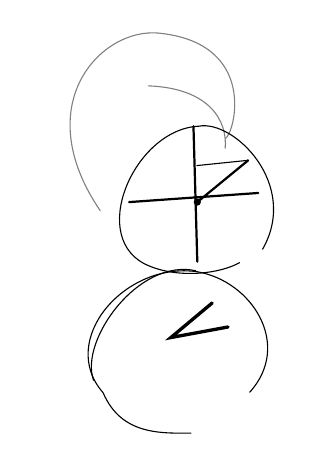
\begin{tikzpicture}[line cap=round,x=.61cm,y=.61cm]
\draw[gray] (-2.0,4.2) .. controls (-3.5,6.4) and (-2,8.0) .. (-.8,7.9) .. controls (1.3,7.7) and (.8,5.8) .. (.6,5.7);
\draw[gray] (-1.0,6.8) .. controls (.3,6.75) and (.65,6.05) .. (.6,5.5);
\draw (1.38,3.4) .. controls (2.15,4.75) and (.78,6.1) .. (.05,5.96) .. controls (-1.3,5.9) and (-2.3,3.58) .. (-.98,3.05) .. controls (-.33,2.78) and (.52,2.9) .. (.90,3.12);
\draw[thick] (.02,3.14)--(-.06,5.96) (.02,4.38)--(1.08,5.25) (-1.4,4.38)--(1.29,4.57);
\draw[thin] (.01,5.14)--(1.08,5.25); \fill (.02,4.38) circle (.075);
\draw (1.11,.42) .. controls (2.0,1.4) and (1.17,2.73) .. (.02,2.93) .. controls (-1.49,3.15) and (-2.9,1.5) .. (-1.94,.41) .. controls (-1.56,-.48) and (-.72,-.43) .. (-.11,-.43);
\draw[thin] (-2.14,.67) .. controls (-2.44,1.5) and (-1.2,3.22) .. (-.01,2.95);
\draw[very thick] (.33,2.28)--(-.53,1.56)--(.66,1.78);
\end{tikzpicture}}
\margin{$\frac{\unsure{2|1|4}\pi}{5}\unsure{>|\to}\frac{\pi}{6}\;?$ \par $\frac{4\pi}{5}\leq\frac{5\pi}{6}$}

$u,v',w'$ vecteurs unitaires
\[
 \begin{aligned}
 u&\perp v'\\
 u&\perp w'
 \end{aligned}
 \qquad v'w'=\cos\tfrac{2\pi}{5}
\]
\[
 \begin{aligned}
 x(\alpha)&=u\cos\alpha+v'\sin\alpha\\
 y(\alpha)&=u\cos\alpha+w'\sin\alpha
 \end{aligned}
\]
\[
 x(\alpha)-u=u(\cos\alpha-1)+v'\sin\alpha
\]
\[
 \begin{aligned}
 \|x(\alpha)-u\|^2&=\|y(\alpha)-u\|^2=(\cos\alpha-1)^2+\sin^2\alpha=2-2\cos\alpha\\
 &=4\sin^2\tfrac{\alpha}{2}\qquad (1-\cos\alpha=2\sin^2\tfrac{\alpha}{2}\\
 \|x(\alpha)-u\|&=2\sin\tfrac{\alpha}{2}\qquad\qquad 1-\cos^2\tfrac{\alpha}{2}+\sin^2\tfrac{\alpha}{2}
 \end{aligned}
\]
\[
 \begin{aligned}
 \|x(\alpha)-y(\alpha)\|^2&=\|v'\sin\alpha-w'\sin\alpha\|^2\\
 &=\sin^2\alpha\;\|v'-w'\|^2=\sin^2\alpha\,(2-2\cos\tfrac{2\pi}{5})\\
 &\deleted{=\sin^2\alpha+\sin^2\alpha-2\cos\tfrac{\unsure{\pi|2\pi}}5\sin^2\alpha}\\
 &=4\sin^2\alpha\sin^2\tfrac{\pi}{\unsure{5|4}}=\deleted{8\sin^2\tfrac{\alpha}{2}\sin^2\tfrac{\alpha}{2}}\;\sin\tfrac{\pi}{5}
 \end{aligned}
\]
\[
 \|x(\alpha)-y(\alpha)\|=2\sin\alpha\sin\tfrac{\pi}{5}
 =4\sin\tfrac{\alpha}{2}\cos\tfrac{\alpha}{2}\sin\tfrac{\pi}{\unsure{4|5}}
\]
\[
 \|x(\alpha)-u\|=\|y(\alpha)-u\|=\|x(\alpha)-y(\alpha)\|
\]
\[
 \Longleftrightarrow\quad 2\cos\tfrac{\alpha}{2}\sin\tfrac{\pi}{5}=1
 \qquad\text{i.e.}\quad \boxed{\cos\tfrac{\alpha}{2}=\frac{1}{2\sin{\pi/5}}}
\]
\margin{\uline{NB} \ $2\sin\frac{\pi}{5}$ = côté du pentagone régulier unité}
% archive sheet number: 17
\scanpage{19}

$G$ groupe d'ordre $60$, opère \inserted{transitivement} sur $I$ ens. d'ordre $15$, sur lequel il y a un autom. $\alpha$ d'ordre $3$ commutant à $G$, d'où $I/\alpha=J$ ens. à $5$ éléments, sur lequel $G$ opère transitivement. Le sous-groupe de stabilité d'un pt \unsure{de|$\in$} $J$ est un sous-groupe \inserted{$F$} d'ordre $12$ de $G$, et on trouve \deleted{que} $G\longrightarrow\unsure{\mathfrak{S}|\mathscr{S}}_5$\inserted{ordre $120$}. Supposons \unsure{pour cela|pour voir|si on sait} que $G$ opère fidèlement sur $J$, alors $G\longrightarrow\mathfrak{S}_5$ est injectif, donc $G\simeq$ sous-groupe d'indice $2$ de $\mathfrak{S}_5$, donc $G\simeq A_5$.

% margin note written sideways
\margin{$\begin{array}{ccc}dD&\longrightarrow&D\\30&&15\\ \alpha'\,?&&\alpha\end{array}$}
% margin note written sideways
\margin{$\alpha'{}^3$ est d'ordre $2$ ou $1$ [\unsure{transfo|transform.} \deleted{\unsure{triviale}} \unsure{correspond} à l'orbite \illegible{2} opposés on a $=$] \par $G/\unsure{H|F|\mathfrak F}_2\longrightarrow G/H_4$}

\figure{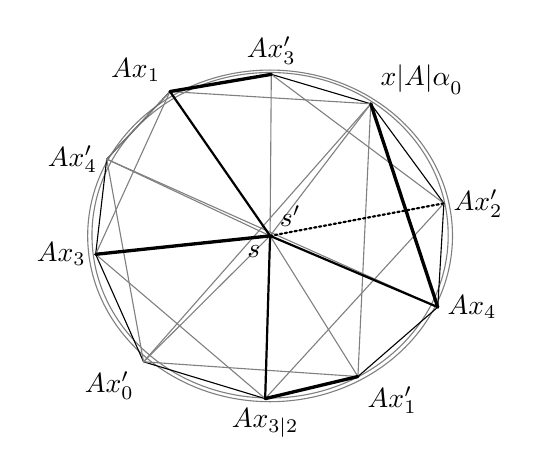
\begin{tikzpicture}[scale=.78,line join=round,line cap=round]
\coordinate (o) at (0,0);
\foreach \nm/\x/\y in {a/1.64/2.15,b/.02/2.63,c/-1.63/2.35,d/-2.66/1.25,e/-2.84/-.30,f/-2.06/-2.05,g/-.08/-2.65,h/1.43/-2.29,i/2.73/-1.16,j/2.83/.53}{\coordinate (\nm) at (\x,\y);}
\draw[gray] (0,0) ellipse (2.97 and 2.70);
\draw[gray] (0,.01) ellipse (2.90 and 2.65);
\draw (a)--(b)--(c)--(d)--(e)--(f)--(g)--(h)--(i)--(j)--cycle;
\draw[gray] (c)--(a)--(h)--(f)--(d)--cycle;
\draw[gray] (b)--(j)--(g)--(e)--(c) (d)--(i) (f)--(a);
\foreach \p in {a,b,d,f,g,h}{\draw[gray] (o)--(\p);}
\draw[thick] (c)--(o)--(i) (o)--(g);
\draw[very thick] (o)--(e) (c)--(b) (a)--(i) (h)--(g);
\draw[densely dotted,thick] (o)--(j);
\node[above right] at (a) {$\unsure{x|A|\alpha}_0$};
\node[above] at (b) {$\deleted{A}x'_3$};
\node[above left] at (c) {$\deleted{A}x_1$};
\node[left] at (d) {$\deleted{A}x'_4$};
\node[left] at (e) {$\deleted{A}x_3$};
\node[below left] at (f) {$\deleted{A}x'_0$};
\node[below] at (g) {$\deleted{A}x_{\unsure{3|2}}$};
\node[below right] at (h) {$\deleted{A}x'_1$};
\node[right] at (i) {$\deleted{A}x_4$};
\node[right] at (j) {$\deleted{A}x'_2$};
\node[below left] at (o) {$s$}; \node[above right] at (o) {$s'$};
\end{tikzpicture}}
\[
 \begin{aligned}
 u&\to u\cos\alpha+v\sin\alpha\\
 v&\to u(-\sin\alpha)+\unsure{v_2|v}\cos\alpha
 \end{aligned}
\]
\figure{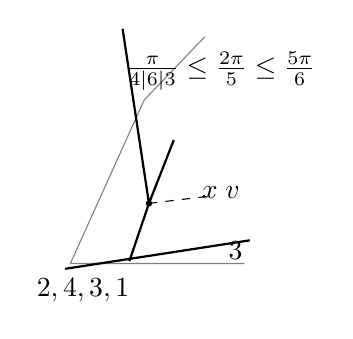
\begin{tikzpicture}[scale=.67]
\draw[thin,gray] (0,0)--(1.4,3.1)--(2.55,4.3) (0,0)--(3.3,0);
\draw[thick] (-.1,-.1)--(3.4,.44) (1.12,.05)--(1.49,1.14)--(1.96,2.34) (1.49,1.14)--(.99,4.45);
\draw[dashed] (1.49,1.14)--(2.74,1.29); \fill (1.49,1.14) circle (.06);
\node[above right] at (.87,3.1) {$\frac{\pi}{\unsure{4|6|3}}\leq\frac{2\pi}{5}\leq\frac{5\pi}{6}$};
\node at (2.85,1.35) {$\deleted{\unsure{x}}\;\unsure{v}$}; \node at (3.13,.25) {$3$};
\node[below] at (.24,-.1) {$2,4,3,1$};
\end{tikzpicture}}
\[
 \alpha'/2=\pi-\tfrac{\alpha}{2}\qquad
 \frac{1}{2\sin^2\theta}-1
\]
\[
 \begin{aligned}
 \cos\alpha&=\cos^2\tfrac{\alpha}{2}-\sin^2\tfrac{\alpha}{2}\\
 &=2\cos^2\tfrac{\alpha}{2}-1\\
 &=1-2\sin^2\theta\\
 &=\cos2\theta
 \end{aligned}
\]
\figure{\begin{tikzpicture}[scale=.56]
\draw (0,0)--(3.9,-.06) (4.2,-.1)--(4.28,2.65) (1.09,.68)--(4.56,1.82);
\node[above] at (2.25,2.03) {$\ell^2=4\sin^2\tfrac{\alpha}{2}$};
\node[rotate=17] at (2.4,1.24) {$2\sin\tfrac{\alpha}{2}\unsure{\cos}$};
\node[right] at (4.2,2.45) {$4$};
\end{tikzpicture}}
\[
 \begin{aligned}
 (AB,A'B')&=P\\
 (EC',CE')&=Q=\alpha(P)\\
 (SD,S'D')&=R=\alpha(Q)=\alpha^2(P)\\
 (AB,A'B')&=\alpha(\unsure{R|P})=\alpha^2(Q)=\alpha^3(P)
 \end{aligned}
\]
\figure{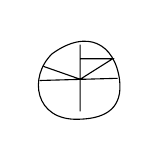
\begin{tikzpicture}[scale=.40]
\draw (0,0) .. controls (-1.4,-.05) and (-1.6,1.35) .. (-.84,2.08) .. controls (.28,2.89) and (1.15,2.39) .. (1.30,1.25) .. controls (1.40,.40) and (.93,.02) .. (0,0);
\draw (.05,.25)--(.05,2.37) (-1.24,1.23)--(1.24,1.30) (-1.12,1.68)--(.05,1.27)--(1.08,1.92)--(.07,1.92);
\end{tikzpicture}}
% margin note written sideways
\margin{$\sigma\in G$, laissant stable $(P,Q,R)$, donc $\sigma\in N$ (\deleted{normalisateur} de Sylow $\simeq\unsure{\mathbb F_2^4|F_2^4}$) l'intersection des conjugués de $N$ est un sous-groupe de $N$, invariant, donc soit $N$, soit $\unsure{\mathbb F|\mathfrak F}_2$, soit $0$. Ce n'est pas $N$, ni $\mathbb F_2$}
% archive sheet number: 18
\scanpage{20}

\figure{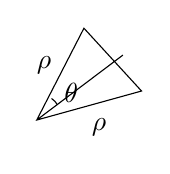
\begin{tikzpicture}[scale=.55]
\draw (0,0)--(1.09,2.12)--(2.42,.67)--cycle (0,0)--(1.99,1.50);
\draw (.48,.35) arc (30:56:.45);
\node at (.8,.63) {$\theta$}; \node[below] at (1.44,.25) {$\rho$}; \node[left] at (.56,1.26) {$\deleted{\unsure{\rho}}$};
\end{tikzpicture}}
\[
 2\rho\sin\tfrac{\theta}{2} \qquad G/H=X\ \underset{e}{\ni}
\]
\figure{\begin{tikzpicture}[scale=.70,line join=round]
\draw[thick] (0,0)--(2.2,3.0)--(2.34,1.0)--(4.93,1.35)--cycle;
\draw[very thick] (0,0)--(2.34,1.0) (2.34,1.0) .. controls (3.24,1.57) and (4.09,1.54) .. (4.93,1.35);
\draw (2.2,3.0) .. controls (2.66,2.33) and (2.51,1.72) .. (2.34,1.0);
\draw[->] (2.34,1.0)--(2.91,2.65); \draw[->] (2.34,1.0)--(3.99,2.01);
\draw[->] (2.22,2.04) .. controls (1.77,1.70) and (.74,2.19) .. (.48,2.88);
\node[left] at (.47,2.87) {$2\sin\tfrac{\alpha}{2}$}; \node at (3.28,2.24) {$72^\circ$};
\node at (1.15,.76) {$1\unsure{\alpha}$}; \node at (1.99,1.92) {$\unsure{\cos}$}; \node at (3.62,.94) {$\cos\alpha$};
\end{tikzpicture}}
\[
 \begin{aligned}
 \cos^2\alpha\cos\tfrac{2\pi}{5}&=\cos\alpha\\
 2\deleted{\unsure{\sin}}\sin\tfrac{\alpha}{2}\sin\tfrac{2\pi}{5}&=1
 \end{aligned}
\qquad
 \boxed{\cos\alpha=\frac{1}{2\sin^2\frac{2\pi}{\unsure{10|5}}}}
\]
\[
 \begin{aligned}
 \unsure{\gamma|y}e&=a.e=\dot a\\
 \gamma x&=\gamma ge=g'ue=g'\unsure{v|u|a}e=\deleted{\unsure{g'}} 
 \end{aligned}
\]
\figure{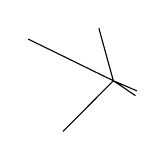
\begin{tikzpicture}[scale=.46]
\draw (0,0)--(2.35,-1.15)--(3,-1.43) (1.95,.30)--(2.35,-1.15)--(2.96,-1.56) (2.35,-1.15)--(.96,-2.55);
\end{tikzpicture}}
\[
 \begin{aligned}
 &\deleted{\unsure{bh}}\qquad b'=bh\\
 &b^{-1}b'\in H\\
 &\Rightarrow (ba)^{-1}b'a\in H\\
 &\text{i.e.}\quad a^{-1}b^{-1}b'a\subset H\\
 &\text{i.e.}\quad a^{-1}Ha\in H
 \end{aligned}
\]
% long diagonal strokes run through the calculation
\[
 1+x+x^2+x^3+x^4=0
\]
% margin note written sideways
\margin{$g(\sigma.i)$
$\begin{array}{ccccc}1&2&3&4&\deleted{5}\\ \hline 2&4&1&3&0\\ \hline 3&1&4&2&0\\ \hline\end{array}$\par
$p(g,\sigma.i)=(p(g),\sigma\unsure{)})(\unsure{\varphi|\rho}(1),\unsure{i})$
\par $\underset{\unsure{E}}{g}(\sigma{i})=g\sigma g^{-1}\quad g\unsure{\sigma'|r'|i}$}
% margin note written sideways
\margin{$\xi\quad\xi^2.\quad u,2u,3u,4u,0 \qquad \xi^i\quad G_{i,0}\quad e^{i\theta}$\par
$\left\{\begin{aligned}u^2+w^2&=1\\[-1pt]&\end{aligned}\right.\quad
\begin{pmatrix}\cos\theta&\unsure{u}\\ &\end{pmatrix}=$\par
$\unsure{\mathrm{II}}\quad\theta^2+\mu^2=1\qquad x^2-y^2$\par
$\begin{array}{ccc} G/\unsure{H} &\longrightarrow&G/H\\ \shortparallel&&\shortparallel\\ X&\longrightarrow&X\end{array}
\qquad \unsure{H}^{\unsure{\varphi}}\subset H$\par
$\begin{pmatrix}u&-v\\v&u\end{pmatrix}=\unsure{q}\begin{pmatrix}1&0\\0&1\end{pmatrix}$}
\figure{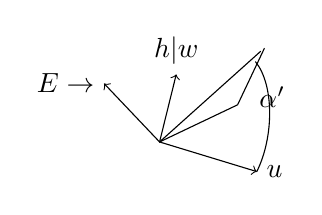
\begin{tikzpicture}[scale=.53,line join=round,line cap=round]
\coordinate (p) at (0,0); \draw[->] (p)--(-1.33,1.4) node[left] {$\unsure{E}\to$};
\draw[->] (p)--(.4,1.62) node[above] {$\unsure{h|w}$}; \draw (p)--(2.42,2.17);
\draw[->] (p)--(2.33,-.71) node[right] {$u$}; \draw (2.33,-.71) .. controls (2.75,.14) and (2.74,1.38) .. (2.30,1.92);
\draw (p)--(1.87,.89)--(2.51,2.24); \node at (2.70,1.07) {$\unsure{\alpha'}$};
\end{tikzpicture}}
\[
 \frac{N(H)}{\bigcap\text{conj.}\,H}\qquad
 \left(2\sin\tfrac{\alpha}{2}\right)\left(2\sin\unsure{>|{}^2} \tfrac{\pi}{4}\right)
\]
\figure{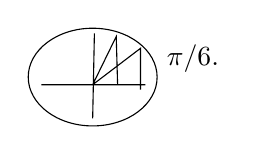
\begin{tikzpicture}[scale=.44]
\draw (0,0) ellipse (1.86 and 1.41);
\draw (0,-1.19)--(.05,1.26) (-1.48,-.22)--(1.52,-.22) (0,-.22)--(1.38,.83)--(1.38,-.36) (0,-.22)--(.68,1.17)--(.72,-.23);
\node[right] at (1.86,.53) {$\pi/6$.};
\end{tikzpicture}}
\[
 \begin{aligned}
 \alpha&=60\,?\\
 \cos\tfrac{\alpha}{2}&=\tfrac{\sqrt3}{2}\\
 \sqrt3\sin\tfrac{\pi}{5}&=1
 \end{aligned}
\]
\figure{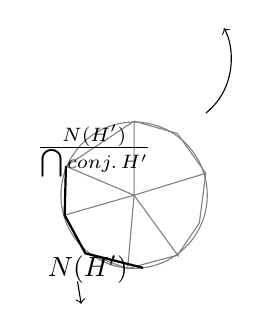
\begin{tikzpicture}[scale=.57, line join=round]
\draw[gray] (0,0) circle (1.63);
\draw[gray] (90:1.65)--(55:1.68)--(17:1.67)--(-23:1.58)--(-54:1.65)--(-95:1.64)--(-130:1.69)--(-164:1.61)--(157:1.65)--cycle;
\draw[gray] (0,0)--(90:1.65) (0,0)--(17:1.66) (0,0)--(-54:1.69) (0,0)--(-95:1.64) (0,0)--(-164:1.61) (0,0)--(157:1.65);
\draw[thick] (157:1.65)--(-164:1.61)--(-130:1.69)--(-83:1.63);
\node at (-.89,.98) {$\frac{N(H')}{\bigcap\text{conj.}\,H'}$}; \node at (-1.03,-1.65) {$N(\unsure{H'})$};
\draw[->] (1.6,1.83) .. controls (2.31,2.4) and (2.23,3.35) .. (2.0,3.72);
\draw[->] (-1.26,-1.92)--(-1.18,-2.42);
\end{tikzpicture}}
\[
 \begin{array}{ccccccc}
 N(H)\cap N(H')&=&N(H\cap H')&\subset&N(H)&=&\mathbb Z_3.\mathbb F_2^2\\
 &&\cup&&\cup\\
 &&H'&\subset&H&\text{---}&\mathbb F_2^2\\
 &&\cup&&\cup\\
 K\cap H'&=&\underset{0}{K'}&\subset&K&=&0
 \end{array}
\]
% archive sheet number: 19
\scanpage{22}

\diagram{\begin{tikzcd}[ampersand replacement=\&,column sep=small,row sep=small]
\mu_5\arrow[d,dash] \& \& I\unsure{\in|\subset|c} Q\arrow[dl]\\
\mu_5^*\arrow[d,dash] \& \unsure{D_5|D'_5|\mathbb V_5}_{\unsure{S|s}}\arrow[d] \&\\
{} \& S\arrow[u,bend left=44]\arrow[dl] \&\\
\mathbb V_5\arrow[d,dash] \& \&\\
\mathbb Z[\frac14] \& \&
\end{tikzcd}}
\[
 \cos'(D_i,D_j)^2+\cos'(D_i,D_j)
\]
$\cos'(D_i,D_j)$ indépendant de $i,j$ pour $i\ne j$. Soit $c$

$c$

a) $\exists$ des icos. loc. \unsure{ét.quement|étliquement} $\forall c$ donné \unsure{où|i.e.} $\boxed{c^2+c-1=0}$

b) Deux icos. \inserted{\unsure{de|$q$} $=c$} sont loc. conjugués par $SO(Q)$

c) Le groupe d'isotropie d'un icosaèdre \inserted{dans $SO(Q)$} (groupe des autom. d'un icosaèdre) est \inserted{fini} étale $/S$, et ses fibres géom. isom. au gr-pe \uline{alterné} à $5$ \uline{lettres}.

\figure{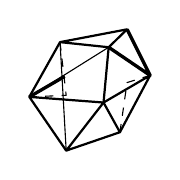
\begin{tikzpicture}[line join=round,scale=.65]
\coordinate (a) at (0,1.05); \coordinate (b) at (.60,2.12); \coordinate (c) at (1.91,2.37); \coordinate (d) at (2.36,1.47); \coordinate (e) at (1.77,.36); \coordinate (f) at (.72,0); \coordinate (g) at (1.45,.94); \coordinate (h) at (1.55,2.02);
\draw[thick] (a)--(b)--(c)--(d)--(e)--(f)--cycle (a)--(g)--(h)--(b) (c)--(h)--(d)--(g)--(f) (e)--(g);
\draw (a)--(h) (b)--(f); \draw[dashed] (b)--(.72,1.08)--(a) (e)--(1.91,1.33)--(d);
\draw[very thick] (c)--(d)--(h) (a)--(.69,1.45);
\end{tikzpicture}}
icosaèdre projectif --- icosaèdre

\figure{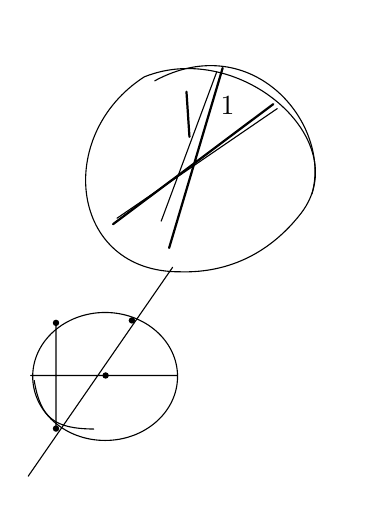
\begin{tikzpicture}[scale=.63,line cap=round]
\draw (.1,1.65) .. controls (-2.13,1.64) and (-2.44,4.41) .. (-.62,5.58) .. controls (1.30,6.35) and (3.66,4.29) .. (2.54,2.83) .. controls (1.95,2.07) and (1.13,1.62) .. (.1,1.65);
\draw (-.41,5.5) .. controls (1.55,6.56) and (3.16,4.64) .. (2.76,3.22);
\draw[thick] (-1.25,2.61)--(1.98,5.03) (-.12,2.13)--(.96,5.76) (.29,4.37)--(.23,5.28);
\draw (-.28,2.67)--(.84,5.68) (-1.17,2.73)--(2.06,4.94); \node at (1.06,5.00) {$1$};
\draw (-1.41,-.46) ellipse (1.46 and 1.29);
\draw (-2.91,-.44)--(.04,-.44) (-2.96,-2.47)--(-.05,1.74) (-2.4,.62)--(-2.4,-1.51);
\draw (-2.84,-.54) .. controls (-2.71,-1.31) and (-2.43,-1.51) .. (-1.64,-1.52);
\foreach \p in {(-2.4,.62),(-.87,.67),(-1.4,-.44),(-2.4,-1.51)}\fill \p circle (.065);
\end{tikzpicture}}
\[
 \begin{gathered}
 1-\unsure{r|\gamma}=r^2\qquad 2-r=1+r^2\\
 r^2+r-1=0\\
 \cos\alpha=\frac{\overset{\cos\alpha}{\deleted{\unsure{a|4}}\,r/2}}{1-r/2}
 =\frac r{2-r}=a+br=\tfrac15(2r+1)=\deleted{\unsure{1/6}}\,\bigl(\tfrac1{\sqrt5}\bigr)
 \end{gathered}
\]
\[
 \begin{aligned}
 \cos2\alpha&=\cos^2\alpha-\sin^2\alpha=2\cos^2\alpha-1=2\frac{r^2}{4-4r+r^2}-1\\
 &=\frac{2(1-r)}{4-4r+1-r}-1\\
 &=\frac{2-2r}{5(1-r)}-1\\
 &=\tfrac25-1=\bigl(-\tfrac35\bigr)\\
 2\cos2\alpha&=-\tfrac65
 \end{aligned}
\]
\[
 \tfrac{2}{25}[4r^2+4r+1]-1\qquad
 \underbrace{4-\deleted{4r}+\deleted{4r}+1}
\]
\[
 \frac{B(x,y)^2}{Q(x)Q(y)}-2=-\tfrac65\ \unsure{2}
 \qquad 2a+(2b-1\inserted{{}-a})r\unsure{-|=|+}br^2=0
\]
\[
 \boxed{B(x,y)^2=\tfrac45 Q(x)Q(y)}
 \qquad r^2+(-2+\tfrac1b+\tfrac ab)r-\tfrac{2a}{b}=0
\]
\[
 -\tfrac{2a}{b}=-1\qquad\boxed{b=2a}\qquad a=\tfrac15\quad b=\tfrac25
\]
\[
 -2+\tfrac{1}{2a}+\tfrac12=1
\]
en car. $2$, \unsure{en effet|cela fait}
\[
 B(x,y)^2=0\qquad \tfrac{1}{2a}=\tfrac52\qquad a=\tfrac15
\]
\[
 \cos'2\alpha=\quad
 2\cos2\alpha=2(2\cos^2\alpha-1)=(2\cos\alpha)^2-2
\]
donc si $2$ \unsure{bon} \deleted{\unsure{alors}} \unsure{si deux}

cela signifie \deleted{$y\perp x$} $y\parallel x$
\[
 \tfrac12 B=B' \qquad \boxed{B'(x,y)^2=\tfrac15 Q(x)Q(y)}
\]
\figure{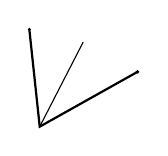
\begin{tikzpicture}[scale=.6]
\draw[thick] (0,2.06)--(.22,0)--(2.29,1.16); \draw (.22,0)--(1.14,1.79);
\fill (0,2.06) circle (.035); \fill (2.29,1.16) circle (.04);
\end{tikzpicture}}
% archive sheet number: 21
\scanpage{23}

\deleted{$E$ topos

$C$ petite Catégorie

alors $\uline{\mathrm{Hom}}\,(C^\circ,E)=\pi(C,E)$ un topos

Si on a des morphismes $C\xrightarrow{f} C'$\quad $g:E\longrightarrow E'$ d'où $g^*:E'\longrightarrow E$, on construit un foncteur $\pi(\unsure{h|f},g):\pi(C,E)\longrightarrow\pi(C',E')$
\[
 \pi(f,g)^*=(u'\longmapsto g^*\circ u'\circ f^\circ),\quad
 \pi(f,g)_*=(u'\longmapsto g_*f_*^{(E)})
\]
\margin{vérifier l'expression donnée de $\pi(f,g)_*$ \ldots}
% slanted
qui est le foncteur image inverse associé à un morphisme de topos
\[
 \pi(f,g):\qquad \pi(C,E)\longrightarrow\pi(\unsure{E|C'},E')
\]
de sorte que $\pi(C,E)$ dépend de façon covariante de $(C,E)$ [on a un 2-foncteur $(\mathrm{Cat})\times(\unsure{\mathrm{Top}|\mathscr{T}op})\longrightarrow(\mathrm{Top})$]

On va définir un morphisme \inserted{de topos} fonctoriel en $C,E$
\diagram{\begin{tikzcd}[ampersand replacement=\&]
\text{\textcircled{1}}\& \pi(C,E)\arrow[d,"{\gamma=\gamma(C,E)}"']\\
\&\widehat C\times_{\mathrm{Top}} E
\end{tikzcd}}
en définissant les composantes
\[
 \begin{aligned}
 \gamma_1=\gamma_1(C,E)&:\quad\pi(\,C,E)\longrightarrow\widehat C\\
 \gamma_2=\gamma_2(C,E)&:\quad\pi(C,E)\longrightarrow E
 \end{aligned}
\]
par
\[
 \gamma_1^*:\quad\underset{\substack{\parallel\\\pi(C,P)}}{\widehat C}
 \longrightarrow\pi(C,E)\qquad\text{défini par}\quad F\longmapsto[X\longmapsto F(X)_E]
\]
\inserted{topos ponctuel}\qquad i.e. $\gamma_1=\pi(\mathrm{id}_C,p_E)$, où $p_E:E\longrightarrow P$ \inserted{``unique'' morphisme de topos}
\[
 \gamma_2^*:\quad\underset{\substack{\unsure{\wr|\parallel|\simeq}\\\pi(C_0,\unsure{P|p|E})}}{E}
 \longrightarrow\pi(C,E)\qquad x\longmapsto(i\longmapsto x)
\]
$\gamma_2^*(x)$ est le foncteur constant de valeur $x$

\inserted{catégorie ponctuelle}\qquad i.e. $\gamma_{\unsure{1|2}}=\pi(p_C,\mathrm{id}_E)$,\quad $p_C:C\longrightarrow C_0$ \inserted{unique morphisme de topos}

\uline{Question} \quad $\gamma(C,E)$ est-il tjrs une équivalence ?

a) \deleted{\unsure{Exemples|Exemple} Supposons} On note que $\pi(C,E)$ transforme sommes en un des deux arguments en sommes, et de même pour $\widehat C\times E$ ($C\longrightarrow\widehat C$ transformant sommes en sommes). Donc on est ramené à traiter le cas $C$ connexe.

b) $C$ un groupoïde --- qu'on peut supposer connexe. Alors $\widehat C\simeq B_G$, $G$ un groupe, $\pi(C,E)\simeq B_{G_E}$ (catégorie des objets de $E$ avec $G$ opérant), ok

c) $E=\widehat D$, alors $\pi(C,E)\simeq\widehat{C\times D}$, et $\gamma(C,E)$ est le morphe. \deleted{fonctoriel}\inserted{de topos} évident
\[
 \widehat{C\times{D}}\longrightarrow\widehat C\times\widehat{D}
\]
}
% archive sheet number: 22
\scanpage{25}

$X$ espace topologique \deleted{compact} $G_1$ [triangulable compact de dim $\leq1$]

$S$ surface \uuline{orientée}

Nous voulons étudier les classes d'isotopie des plongements (modérés\ldots.) $X\xrightarrow{\varphi}S$.

Pour tout tel plongement\inserted{$\varphi$}, et pour tout sommet \deleted{de} \inserted{topologique} non isolé de $X$, il y a un \uline{ordre circulaire}\inserted{$\omega_x(\varphi)$} sur l'ens des arêtes (orientées) issues de $x$ induit par $\varphi$ \deleted{de} [donnée vide si le sommet $x$ est un bout, i.e. s'il n'y a qu'une seule arête issue de $x$ ; sinon, il y \deleted{a \unsure{un entier} \illegible{1}} a $\unsure{\nu|v}_x\geq3$ telles arêtes, et \deleted{le nombre de} l'ens des ordres circulaires possibles est un ens. $\Omega_x(X)$ à $(\nu_x-1)!$ éléments).

On trouve ainsi un premier invariant
\[
 \omega(\varphi)=(\omega_x(\varphi))_{x\in X'_0}\in\prod_{x\in X'_0}\Omega_x(X)
\]
\inserted{ens. des sommets de $X$ qui ne sont ni isolés ni des bouts}

On a une appl.
\[
 \mathrm{Pl}_{\mathrm{isot}.}(X,S)\xrightarrow{\omega}
 \prod_{x\in\unsure{x|X}'_0}\Omega_x(X)\overset{\text{déf}}{=}\Omega(X)
\]
et notre propos est d'étudier les fibres \inserted{$\mathrm{Pl}_{\mathrm{isot}}^\alpha(X,S)$} de $\omega$, plus précisément, pour $X$ et un $\alpha=(\alpha_x)_{x\in X'_0}\in\deleted{\unsure{\prod\Omega_x}}\Omega(X)$ fixés, d'étudier pour tt $S$ les plongements $\varphi:X\hookrightarrow S$ tels que $\omega(\varphi)=\alpha$.

Pour ceci, \deleted{\unsure{notons le}} \deleted{D}définissons pour tt \unsure{plongement} ``le'' voisinage tubulaire \inserted{fermé} relatif à celui-ci. On trouve

\uline{Th 1} Pour $\alpha$ fixé, ce voisinage tubulaire \deleted{est \unsure{défini} \illegible{1}}\inserted{ne dépend}, à homéomorphismes près induisant l'identité $X$ [de façon \unsure{lui-même|unique} à isotopie près] que de $\alpha$, soit $\unsure{U|\mathcal U}_\alpha$, et non de $S$. \deleted{\unsure{L'on|Donc}} On trouve alors une application
\[
 \mathrm{Pl}_{\mathrm{isot}}^\alpha(X,S)\longrightarrow\mathrm{Pl}_{\mathrm{isot}}(U_\alpha,S)
\]
Celle-ci est une bijection
% archive sheet number: 24
\scanpage{26}

Ce théorème ramène essentiellement l'étude de $\mathrm{Pl}_{\mathrm{isot}}^\alpha$ à celle de $\mathrm{Pl}_{\mathrm{isot}}(U_\alpha,S)$. Pour faire cette étude, on doit pouvoir donner un procédé pour décrire combinatoirement $U_\alpha$ en termes de $\alpha$. Notons

\uline{Prop} $U_\alpha-X=\unsure{V|W|\mathcal V}_\alpha$ a des composantes connexes \inserted{$V_\alpha^i$} qui sont des produits $\underset{\text{cercle}}{S^1}\times\deleted{\unsure{]0,1[}}[1,2[$ \deleted{et \unsure{$V_\alpha$} \illegible{1} le bord de $U_\alpha$ est le filtre des} \inserted{avec $\mathrm{bord}(U_\alpha)\cap V_\alpha^i\simeq S^1\times\{1\}$}, les voisinages de $X$ dans $U_\alpha$ induisant sur $V_\alpha^i$ le filtre des voisinages de $S^1\times\{1\}$ dans $S^1\times]0,2[$.

% slanted
\margin{le nb des $V_\alpha^i$ est $b_1(X)+1$ si $X$ connexe non vide ? Cela donnerait $b_1(X)+b_0(\unsure{x|X})$ dans le cas général ?}
\figure{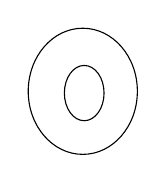
\begin{tikzpicture}[scale=.45]
\draw (0,0) ellipse (1.54 and 1.78); \draw (.04,-.05) ellipse (.56 and .78);
\end{tikzpicture}}
\deleted{Donc}\quad\deleted{\unsure{Déf}}

Donc la surface $S$, pour un plongement donné de $U_\alpha$, peut se décrire comme \deleted{\unsure{$U_\alpha$|$\mathcal U_\alpha$}} déduite de $U_\alpha$ en lui collant une variété \inserted{orientée} à bord $U'$ [compacte \unsure{sss|ssi} $S$ est compacte] \deleted{\unsure{à|---}} savoir $\overline{S-\varphi(U_\alpha)}$ --- à $U_\alpha$, par un isom \deleted{\unsure{de}} $bU'_{\unsure{\alpha}}$ avec $-bU_\alpha\simeq$

\figure{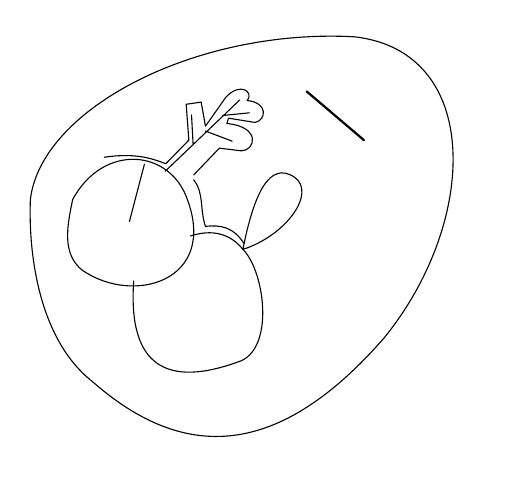
\begin{tikzpicture}[scale=.68,line cap=round,line join=round]
\draw (-3.4,.70) .. controls (-3.2,2.4) and (-.3,3.9) .. (2.65,3.74) .. controls (5.05,3.47) and (4.97,.29) .. (3.21,-1.88) .. controls (1.25,-4.13) and (-.51,-4.22) .. (-2.24,-2.70) .. controls (-3.21,-1.94) and (-3.44,-.40) .. (-3.4,.70);
\draw (-2.61,.70) .. controls (-2.04,1.76) and (-.78,1.65) .. (-.46,.68) .. controls (.08,-.82) and (-1.47,-1.28) .. (-2.43,-.62) .. controls (-2.82,-.31) and (-2.71,.22) .. (-2.61,.70);
\draw (-1.47,-.82) .. controls (-1.58,-2.4) and (-.87,-2.84) .. (.54,-2.31) .. controls (1.16,-2.03) and (.97,-.63) .. (.57,-.23) .. controls (.28,.13) and (-.10,.12) .. (-.41,.02);
\draw (.57,-.23) .. controls (1.38,.03) and (1.95,.83) .. (1.53,1.12) .. controls (1.06,1.43) and (.77,.79) .. (.57,-.23);
\draw (-1.27,1.36)--(-1.55,.29);
\draw (-2.02,1.49) .. controls (-1.37,1.59) and (-1.05,1.43) .. (-.87,1.37) --(-.44,1.81)--(-.49,2.48)--(-.21,2.52)--(-.13,2.07)--(.25,2.61) .. controls (.53,2.91) and (.78,2.70) .. (.65,2.55) .. controls (1.04,2.51) and (1.01,2.19) .. (.80,2.14)--(.30,2.22)--(.27,2.12) .. controls (.92,2.06) and (.80,1.61) .. (.54,1.61)--(.13,1.66)--(-.35,1.16);
\draw (-.88,1.23)--(.51,2.56) (-.36,1.72)--(-.39,2.28) (-.13,1.98)--(.37,1.79) (.19,2.27)--(.69,2.32);
\draw (-.35,1.07) .. controls (-.15,.81) and (-.24,.52) .. (-.13,.20) .. controls (.15,.23) and (.39,.19) .. (.59,-.12);
\draw[thick] (1.76,2.72)--(2.83,1.81);
\end{tikzpicture}}
\figure{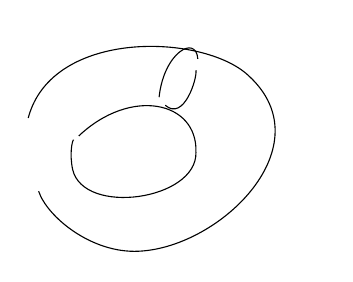
\begin{tikzpicture}[scale=.60]
\draw (-2.45,.63) .. controls (-1.95,2.53) and (1.28,2.42) .. (2.22,1.52) .. controls (3.82,.05) and (1.63,-2.11) .. (-.11,-2.19) .. controls (-1.11,-2.24) and (-2.05,-1.46) .. (-2.23,-.92);
\draw (-1.38,.25) .. controls (-.28,1.29) and (1.14,.99) .. (1.10,-.10) .. controls (1.12,-1.11) and (-1.28,-1.45) .. (-1.51,-.46) .. controls (-1.58,-.13) and (-1.52,.15) .. (-1.49,.17);
\draw (.32,1.07) .. controls (.42,2.02) and (1.10,2.40) .. (1.14,1.88) (.45,.90) .. controls (.85,.55) and (1.13,1.48) .. (1.10,1.64);
\end{tikzpicture}}
\uline{Le Pb} de trouver $\mathrm{Pl}_{\mathrm{isot}}^\alpha(S)$ étant lié à celui de trouver, à \unsure{homéom.|isom.} près\inserted{induisant l'ident. sur $X$}, \deleted{\unsure{près|tous}} les plongements \deleted{près} de $X$ dans une surface \deleted{\unsure{non}} orientée, on peut déjà envisager la solution de ce Pb : il s'agit de trouver les façons possibles d'écrire $J\times S^1$ ($J$ \inserted{$=\pi_0(V_\alpha)$} étant l'ens. d'indices fini discret comme opposé du bord orienté d'une surface à bord [connexe \deleted{\unsure{et une}} ou non] [\deleted{NB $\overline M$ si $U'_\alpha$ est connexe, \unsure{connexe} \inserted{et tte} composante connexe de \deleted{\unsure{$G$}} $U'_\alpha$ \deleted{\unsure{a de}} rencontre le bord \deleted{\unsure{de}} alors $S$ est \unsure{co} (et \unsure{si, sauf si})} $S$ est connexe.

\margin{\uline{NB} $U'_\alpha$ n'est pas connexe en général, mais on peut supposer que tte composante connexe a un bord ($\sim$ tte comp. connexe de $S$ rencontre $X$)}

Donc la classification est donnée aussi \unsure{ici|\{} si relativement aux $U'$ qui est le cas
% archive sheet number: 25
\scanpage{27}

a) On donne une partition \inserted{$\pi$} de $J$ en parties $(J_\lambda)_{\lambda\in\Lambda}$

b) Pour tout $\lambda$, on donne une \deleted{\unsure{variété}} surface orientée \inserted{connexe} à bord $U'_\lambda$, et un isom $bU'_\lambda\simeq-J_\lambda\times S^1$. Si on se borne aux $S$ ``\unsure{algébrique|algébriques}'' (compacte moins ens fini) Une telle $U'_\lambda$ sera connue quand on connait

a) le genre \inserted{$g_\lambda$} de la surface compacte sans bord obtenue en ``rajoutant les points à l'infini'' (i.e. les bouts) et en contractant chaque composante du bord en un point

b) le nb de bouts $\unsure{\beta|\nu}_\lambda$ de $U'_\lambda$.

[\uline{NB} Comme il y aura tjrs un homéom. \inserted{orienté} de $U'_\lambda$ sur lui-même \deleted{identique, \unsure{ou} isotope à l'identité} qui échange entre eux de façon prescrite les éléments du bord, on n'a pas à s'en faire pour préciser la \deleted{\unsure{nat}} correspondance entre \deleted{\unsure{pts}} \inserted{composantes} du bord et les \deleted{\unsure{éléments} de $J_\lambda$} \inserted{élém. de $J_\lambda$} \deleted{\unsure{ou}}]

En fait, en termes de $g_\lambda$, $\beta_\lambda$ on construit $U'_\lambda$ en prenant la surface \deleted{\unsure{algébr.}}\inserted{sans bord} orientée $\unsure{S}$ compacte de genre $g$, soit $S_g$, on y prend $J_\lambda$ rondelles disjointes $D_j$ ($j\in J_\lambda$), et \deleted{\unsure{un}}\inserted{une} partie \deleted{$\beta_\lambda$ points de} finie $\unsure{\Phi|P}_\lambda$ de cardinal $\beta_\lambda$ ne rencontrant pas $\bigcup_{j\in J_\lambda}D_j$, et prend $U'_\lambda=S_g-\bigcup_{j\in J_\lambda}D_j^\circ-\Phi_\lambda$
% slanted
\margin{$S$ compacte $\unsure{\Leftrightarrow}$ les $U'_\lambda$ cpcts, i.e. les $\unsure{\nu|\beta}_\lambda=0$}

Soit $S_{\alpha,\pi,g,\beta}$ la surface ainsi construite à l'aide de
\[
 \left\{\begin{aligned}
 &\alpha\in\Omega(X)\quad[\text{d'où }J=J(\alpha),\text{ à expliciter combinatoirement}]\\
 &\pi\text{ partition de }J\text{ en }(J_\lambda)_{\lambda\in\Lambda}\\
 &(g_\lambda)_{\lambda\in\Lambda}\in\deleted{\unsure{\mathbb N^{*\Lambda}}}\,\mathbb N^\Lambda\\
 &(\beta_\lambda)_{\lambda\in\unsure{J|\Lambda}}\in\deleted{\unsure{\mathbb N^{*\Lambda}}}\,\mathbb N^\Lambda
 \end{aligned}\right.
\]
On a donc un plongement canonique
\[
 X\lhook\joinrel\xrightarrow{\varphi_{\alpha,\pi,g,\beta}} S_{\alpha,\pi,g,\beta}
\]
\margin{\uline{NB} $S_{\alpha,\pi,g,\nu}$ aura $\nu=\sum_\lambda\nu_\lambda$ bouts. Il faut calculer son genre, il doit \deleted{être}\inserted{quelque chose comme} $\sum_{\lambda\in\Lambda}g_\lambda+\gamma(\alpha)$, $\gamma(\alpha)$ un entier (le genre de $U_\alpha$) \uuline{vérifier}}

On trouve donc

\uline{Th 2} Tout plongement $X\longrightarrow S$ \inserted{($S$ surface orientée \uline{algébrique})} est isomorphe à un $\varphi_{\alpha,\pi,g,\beta}$ pour $\alpha,\pi,g,\beta$ convenables, uniquement déterminé
% archive sheet number: 26
\scanpage{28}

Donc on trouve, \deleted{pour} $S$ fixé, une application
\[
 \mathrm{Pl}_{\mathrm{isot}}(X,S)\longrightarrow
 \begin{gathered}\text{Ensemble des systèmes}\\
 \alpha,\pi,g,\nu\ \text{associés à }X\quad(\text{à expliciter}\\
 \text{combinatoirement})\end{gathered}
\]
et on est donc ramené à étudier, pour $\rho=\alpha,\pi,g,\nu$ fixé l'ens des $\mathrm{Pl}_{\mathrm{isot}}(X,S;\rho)$ qui correspondent à ce $\rho$ (non vide sss $S\simeq S_\rho\overset{\text{déf}}=S_{\alpha,\pi,g,\nu}$). \margin{ce qu'on va supposer dorénavant} Or on a une application \deleted{\unsure{Isotopt|Isot}} ``restriction à $X$
\[
 \boxed{\mathrm{Isot}(S_\rho,S)\xrightarrow{r}\mathrm{Pl}_{\mathrm{isot}}(X,S;\rho)}
\]
\inserted{\unsure{préservant|et précisé} orientation\ldots.} qui, d'après ce qu'on vient de voir, est \uline{surjective}.

\deleted{Il reste à}

\deleted{b) étudier quelles sont les fibres de cette application, \deleted{i.e.}

a) Déterminer l'ens $\mathrm{Isot}(S_\rho,S)$

La question a) est classique et résolue : $\mathrm{Isot}(S_\rho,S)$ est un torseur \inserted{à dr} sous $\mathrm{Autext}(\pi_1(S_\rho))$ \inserted{(ou à g. sous $\mathrm{Autext}(\pi_1(S))$)} [du moins si $S_\rho$ est compacte i.e. $\sum_{\lambda\in\Lambda}\unsure{\nu|\lambda}_\lambda=0$ i.e. les $\nu_\lambda$ nuls \ldots]. \deleted{Donc la question est la suivante}

Soit $f:S_\rho\xrightarrow{\sim} S_\rho$ un homéomorphisme, dont la classe d'homotopie est déterminée par l'\deleted{\unsure{endom}}\inserted{extérieur} induit par $f$ sur $\pi_1(S_\rho)=G_\rho$, \deleted{soit \unsure{$E(f)$}} \inserted{soit $E(f)\in\mathrm{Autext}(G_\rho)$}, considérons $f|X=f_X$. Quelle condition sur $E(f),E(g)$ assurent que $f_X\overset{\mathrm{isot}}{\simeq}g_X$ ?}

\diagram{\begin{tikzcd}[ampersand replacement=\&,row sep=small,column sep=small]
G_\rho\arrow[r,shift left=.55ex,"{\bar f,\bar g}"]\arrow[r,shift right=.55ex]\&G_\rho\\
\pi_1(X)\arrow[u]\arrow[ur,bend right=48,dash]\&
\end{tikzcd}}
\uline{NB} Notons que le premier
\[
 G=\mathrm{Isot}_{\mathrm{or}}(S,S)\qquad[\simeq G_\rho\simeq\mathrm{Isot}_{\mathrm{or}}(S_\rho,S_\rho)]
\]
opère sur les deux mbres de $(*)$, et que $r$ commute à l'opération de ce groupe. D'autre part, \deleted{on sait}\inserted{il est clair} que le premier mb est un torseur sous $G$, donc, choisissant $f:S_\alpha\simeq S$, \unsure{et si|si} $r(f)=f_X=f|X$ est son image, et $H$ son stabilisateur, on a que $r$ s'identifie à l'application $G\longrightarrow G/H$. Donc on
% archive sheet number: 27
\scanpage{29}

est finalement ramené aux $2$ questions suivantes

a) Déterminer $G=\mathrm{Isot}(S,S)$

b) Déterminer le sous-groupe \inserted{$H$} de $G$ formé des $h:S\longrightarrow S$ tels que $h\circ f|X\overset{\mathrm{isot}}{\simeq}f$.

On peut \unsure{évidemt|évidemment} supposer $S=S_\rho$ donc $G=G_\rho$, et $f=\varphi_\rho:X\longrightarrow S_\rho$, donc la question devient

a) Déterminer $G_{\unsure{S|\rho}}=\mathrm{Isot}(S_\rho,S_\rho)$ \inserted{$S_\rho$ surface de genre \deleted{\unsure{$g$}} $\unsure{\gamma}$ moins $\unsure{\nu|v}'$ pts \ldots}

b) Déterminer le sous-groupe $H_S\subset G_S$ des $h\in G_\rho$ tels que
\[
 \deleted{h|X\simeq}\qquad h\circ\varphi_\rho\simeq\varphi_\rho
\]
Tout dépend seulement du couple $X\subset S_\rho=S$, \deleted{\unsure{un}} surface orientée avec $\unsure{x|X}$ \inserted{connexe} un $X$ compact ($\in\mathrm{Ob}\,G_1$) plongé dedans.

La réponse à a) est classique (du moins si $S_\rho$ compact) \deleted{$G$ est} l'homomorphisme can
\[
 G\longrightarrow\mathrm{Aut\,ext}(\pi_1(S,s))
\]
est un Isom, et $G$ est donc le \uline{groupe de Teichmuller} de \deleted{\unsure{$S_\alpha$}} $S$. Reste à trouver (pour un $X\underset{\varphi}{\subset} S$ plongé dans $S$) quels sont les $h\in G$ tels que $h\circ\varphi\deleted{\unsure{x}}\underset{\mathrm{isot}}{\simeq}\varphi$.

\uline{Cas particulier} \inserted{$X$ connexe et} $\pi_1(X)\longrightarrow\pi_1(S)$ surjectif (sauf erreur, cela signifie \inserted{la partition \inserted{$(J_\lambda)$} de $J$ est discrète ($\Lambda=J$) et} que les $g_\lambda$ et les $\nu_\lambda$ sont nuls --- i.e. que $S_\rho$ est déduite de $\rho$ simplement en ``bouchant séparément chaque trou par une rondelle'' : plongements \uline{normaux}$^*$. Alors
% slanted
\margin{\unsure{pas} tout à fait vrai \unsure{sauf} peut-être. à vérifier\ldots.}
\[
 h\circ\varphi\underset{\mathrm{isot}}{\simeq}\varphi\quad\Longrightarrow\quad
 h\circ\varphi\underset{\mathrm{homot}}{\simeq}\varphi\qquad\text{donc}
\]
\diagram{\begin{tikzcd}[ampersand replacement=\&,row sep=small]
\pi_1(X)\arrow[r,"c"]\arrow[dr]\arrow[d,dash]\&\pi_1(S)\arrow[d,"\pi_1(h)"]\\
{}\&\pi_1(S)
\end{tikzcd}}
$\pi_1(h)\circ c=c$ mod autom \unsure{intérieurs|extérieurs}, donc $\pi_1(h)$ est un autom intérieur, $c$ étant surjectif, on \uline{gagne}.

Cela nous donne en particulier les plongts de \inserted{$X$ \uline{connexe}} dans $S^1$ (car tt \deleted{\unsure{plongt|plongement}} \inserted{\unsure{hom.|homéom.} orienté} de $S^1$ sur lui-mê est isotope à l'identité). Ils sont classifiés par les $\alpha$ tels que $\gamma(\alpha)$ [le genre de $\widetilde U_\alpha$ déduit de $U_\alpha$ par le procédé dit qui donne \deleted{\unsure{des}} un
% archive sheet number: 28
\scanpage{30}

plongement normal) $=0$. Il faut donner un critère simple sur $\alpha$ pour qu'il en soit ainsi.

\uline{Question} Supposons que $h\in G$ soit tel que pour tte composante connexe $X_i$ de $X$, désignant par $\varphi_i:X_i\longrightarrow S$ le plongmt induit, $\pi_1(\deleted{\varphi}h\varphi_i)=\pi_1(h)\circ\pi_1(\varphi_i)\in\deleted{\unsure{\mathrm{Homext}}}\inserted{\mathrm{Hom\,ext}}(\pi_1(X_i),\pi_1(S))$ soit \unsure{égal|égale} à $\pi_1(\varphi_i)$, \deleted{Alors a-t-on} (condition évidemment nécessaire pour que \deleted{\unsure{$f$}} $h\circ\varphi$ soit \unsure{isoto|isot|isotope} à $\varphi$, \deleted{donc} i.e. $h\in H$) ; alors \unsure{à-t-on|a-t-on} $h\in H$ ?
% archive sheet number: 29
\scanpage{31}

\[
 \unsure{\mathscr{G}|\mathcal G}/\unsure{\mathscr{H}|\mathcal H}\simeq\unsure{\mathrm{I}|X|\mathfrak X}
\]
\[
 \pi_1(\mathscr H)\unsure{\text{---}|\longrightarrow}\,
 \overbrace{\pi_{\unsure{1|2}}(\mathscr G)\text{---}\pi_1(\mathrm I)\unsure{\text{---}|\longrightarrow}
 \pi_0(\mathscr H)\longrightarrow\pi_0(\mathscr G)\longrightarrow\pi_0(\mathrm I)}^{??}
\]
\[
 \deleted{\unsure{\pi_1(\mathscr G)\longrightarrow\pi_1(\mathscr H)|\pi_1(\mathcal G)\longrightarrow\pi_1(\mathcal H)}}
\]
\inserted{ens les $h$ tels que $h|X=\text{\unsure{identité|identᵗᵉ}}$}

$\mathscr H=\mathrm{Aut}(S/X)$

\inserted{groupe top.}
% archive sheet number: 30
\scanpage{33}

\deleted{Graphe
\diagram{\begin{tikzcd}[ampersand replacement=\&,column sep=small,row sep=small]
(S,\arrow[d]\&A,\arrow[d]\&R,\arrow[d]\&\sigma)\arrow[d]\&R\subset S\times A\\
\text{sommets}\&\substack{\text{arêtes}\\\text{\unsure{orientées|orientée}}}\&\substack{\text{relation}\\\text{\unsure{incidence}}}\&\text{symétrie}\&
\end{tikzcd}}}
\deleted{Graphe $S$ : ensemble $S$ avec une partie $A$ de $S\times S$, stable par symétrie}

Graphe
\[
 (S,A,A'\xrightarrow{\varphi=(\varphi_1,\varphi_2)=(\varphi_1,\varphi_1\circ\sigma)}S\times S,\sigma)
 \Longleftrightarrow (S,R\subset A\times A,L\longrightarrow A,\sigma)
\]
\diagram{\begin{tikzcd}[ampersand replacement=\&,row sep=small,column sep=small]
 S\arrow[d]\&A\arrow[d]\&A'\arrow[d,bend right=15]\&\varphi\arrow[d]\&\sigma\arrow[d]\\
 \text{sommets}\&\substack{\text{arêtes}\\\text{orientées}}\&\substack{[\text{arêtes}\\\text{non circulaires isolées}]}\&\substack{\deleted{\text{\unsure{symétrie}}}\\\deleted{\text{\unsure{départ}}}}\&\substack{\text{symétrie}\\\text{dans }A}
\end{tikzcd}}
\inserted{$R$ stable par sym.\qquad $L$ arêtes \unsure{boucles|bouclées}}

$G$ groupe des symétries du graphe \qquad $G\simeq\mathrm{Perm}^{\unsure{\prime}}(S)\times\mathrm{Perm}(A)$

Supposons que $G$ est transitif sur $A$ et sur $S$.

Alors a) \deleted{tous les \unsure{pts}} ou bien tous les \deleted{points}\inserted{sommets} sont isolés (et les arêtes sont circulaires isolées) donc le graphe est juste formé de deux ensembles $S,A$, $A'=\varnothing$, et un autom d'ordre $2$ dans $A$ \deleted{\unsure{commutant à}}\inserted{sans pt fixe}. \deleted{l'action de $G$. Donc}
\[
 \mathrm{Aut}\,\Gamma=\mathrm{Perm}(S)\times\mathrm{Aut}(A,\sigma)
\]
% slanted
\margin{tous les sommets isolés}

\margin{Si $A_{1}=A/\sigma$, on trouve que $\mathrm{Aut}(A,\sigma)\simeq\mathrm{Perm}(A_1).(\mathbb Z/2\mathbb Z)^{A_1}$ Ceci doit \unsure{servir|revenir|semi} d'\unsure{int|intro|direct}}

\deleted{[b) ou bien \inserted{il y a des sommets non isolés, donc} tous les sommets sont non isolés, \deleted{et il y a des points \unsure{et donc}} Dans ce cas, il y a des arêtes non \inserted{circulaires} isolées, \deleted{ou bien} toutes les arêtes sont non \inserted{circulaires} isolées [car il y en a non isolées]

% slanted
\margin{il existe des arêtes non isolées circulaires}

\deleted{Il est possible} Ou bien toutes les arêtes sont circulaires, donc $\varphi$ se réduit à une application \uline{surjective}
\[
 \varphi:A\longrightarrow S
\]
compatible avec $\sigma$ $[\varphi\sigma x=\varphi x]$

\deleted{On aura $A$} Choisissons $a\in A$, donc $A\simeq G/G_a^{\inserted{=H}}$ (groupe d'isotropie) et si $s=\varphi(a)$, $S\simeq G/G_s^{\inserted{=H'}}$, $\underset{\unsure{H'}}{G_s}\supset\unsure{A|H|G_a}$ : L'application $\sigma:A\longrightarrow A$ correspond à la donnée d'un élément de $\dot\sigma\in\mathrm{Norm}(G_a)/G_a$, $\dot\sigma$ d'ordre $2$ ; le fait que $\unsure{\rho|\varphi}$ \deleted{\unsure{commute}}\inserted{est compatible} avec $\sigma$ signifie que $\sigma\in G_s=H'$ ; le fait que $\sigma$ opère sans pts fixes signifie que $\sigma\notin H\deleted{\unsure{\bigcup_{g\in G}gHg^{-1}}}$ ; donc on a
\[
 \left\{\begin{aligned}
 &\boxed{G\supset H'\supset H}\quad\text{et}\\
 &\deleted{\sigma\in H'\cap\mathrm{Norm}_G(H)\cap\complement(\unsure{\bigcup_{g\in G}gHg^{-1}})H}\\
 &\boxed{\dot\sigma\in(H'\cap\mathrm{Norm}_G(H))/H\qquad\dot\sigma^2=1,\ \dot\sigma\ne1}
 \end{aligned}\right.
\]
Le fait que $G$ opère fidèlement \inserted{sur $\Gamma$} signifie que
\[
 \bigcap_{g\in G}gHg^{-1}=\{1\}
\]
Si on a une telle situation \hfill ]}
% archive sheet number: 32
\scanpage{34}

c) Ou bien il y a des \unsure{arrêtes|arêtes} non circulaires, donc ttes les arêtes sont non circulaires, on trouve alors
% slanted
\margin{il existe des arêtes non circulaires}
\[
 \underset{\substack{\rotatebox{90}{$\in$}\\a}}{A}
 \mathrel{\mathop{\longrightarrow}^{\varphi_1}_{\text{source}}}
 \underset{\substack{\rotatebox{90}{$\in$}\\s}}{S},\quad
 \left\{\begin{aligned}
 &\sigma:A\unsure{\text{---}|\longrightarrow}A\\
 &\sigma^2=\mathrm{id},\quad\sigma\ \text{ss pt fixe}
 \end{aligned}\right.
\]
\[
 \boxed{G\supset\underset{\substack{\parallel\\G_a}}{H'}\supset
 \underset{\substack{\parallel\\G_s}}H\qquad
 \dot\sigma\in\mathrm{Norm}_G(H)/H\qquad\dot\sigma^2=1\quad\dot\sigma\ne1}
\]
Si on veut que $G$ opère fidèlement, on \deleted{\unsure{pourra}} doit avoir
\[
 \boxed{\bigcap_{g\in G}g^{\deleted{\unsure{\mathrm{au}|-1}}}Hg^{-1}=\{1\}}
\]
Exprimons la condition que $\deleted{\forall}\;\varphi:A\longrightarrow S\times S$ est injectif [donc que $\Gamma$ est un ``schéma simplicial de dim $1$'', donné par un ens. de parties de cardinal $2$ de l'ens. $S$]

C'est l'application
\[
 \begin{aligned}
 G/H&\longrightarrow G/H'\times G/H'\\
 gH&\longmapsto gH',g\sigma H'
 \end{aligned}
\]
donc à prouver que si $g,g'\in G$ tels que $g'{}^{-1}g\in H',\ \sigma^{-1}(g'{}^{-1}g)\sigma\in H'$ alors $\deleted{\unsure{H}}\;g'{}^{-1}g\in H$, i.e.
\[
 \boxed{H'\cap\dot\sigma^{-1}H'\dot\sigma\subset H}
\]
% archive sheet number: 33
